\documentclass[10pt,xcolor={usenames,dvipsnames}]{beamer}
\graphicspath{{pics/}}
\fontfamily{pnc}
\usepackage{verbatim}

\title{Final Presentation}
\subtitle{MyTaxiService}
\author{Roberto Clapis, Erica Stella}
\institute{Politecnico di Milano}
\date{12/02/2016}
\subject{Software Engineering 2}

\usepackage{graphicx}
\usebackgroundtemplate{
\includegraphics[width=\paperwidth,height=\paperheight]{background2.jpg}}

\setbeamercolor{frametitle}{fg=CornflowerBlue}
\setbeamercolor{title}{fg=CornflowerBlue}
\setbeamercolor{framesubtitle}{fg=RoyalBlue}

\addtobeamertemplate{frametitle}{\vskip+3ex}{} %chktex 20

\begin{document}
\frame{\titlepage}
\begin{frame}
	\frametitle{Table of Contents}
	\tableofcontents[currentsection]
\end{frame}


\section[Section]{RASD}

\begin{frame}
	\begin{center}
		RASD	
	\end{center}
\end{frame}
\begin{frame}
	\frametitle{The RASD Document}
	\framesubtitle{The approach}
	We tried to solve all the easy problems with a KISS approach, in order to focus on the actual difficulties. \\
	\begin{itemize}
		\item Login, logout, registration were kept as standard as possible
		\item Usability was kept in mind, customizability was not considered as a feature
		\item We tried to keep as little as possible the user inputs and let the application do the work
	\end{itemize}
\end{frame}
\begin{frame}
	\frametitle{Two simple interfaces}
	\framesubtitle{Adaptive web-based UI to ensure maintainability}
	\begin{center}
		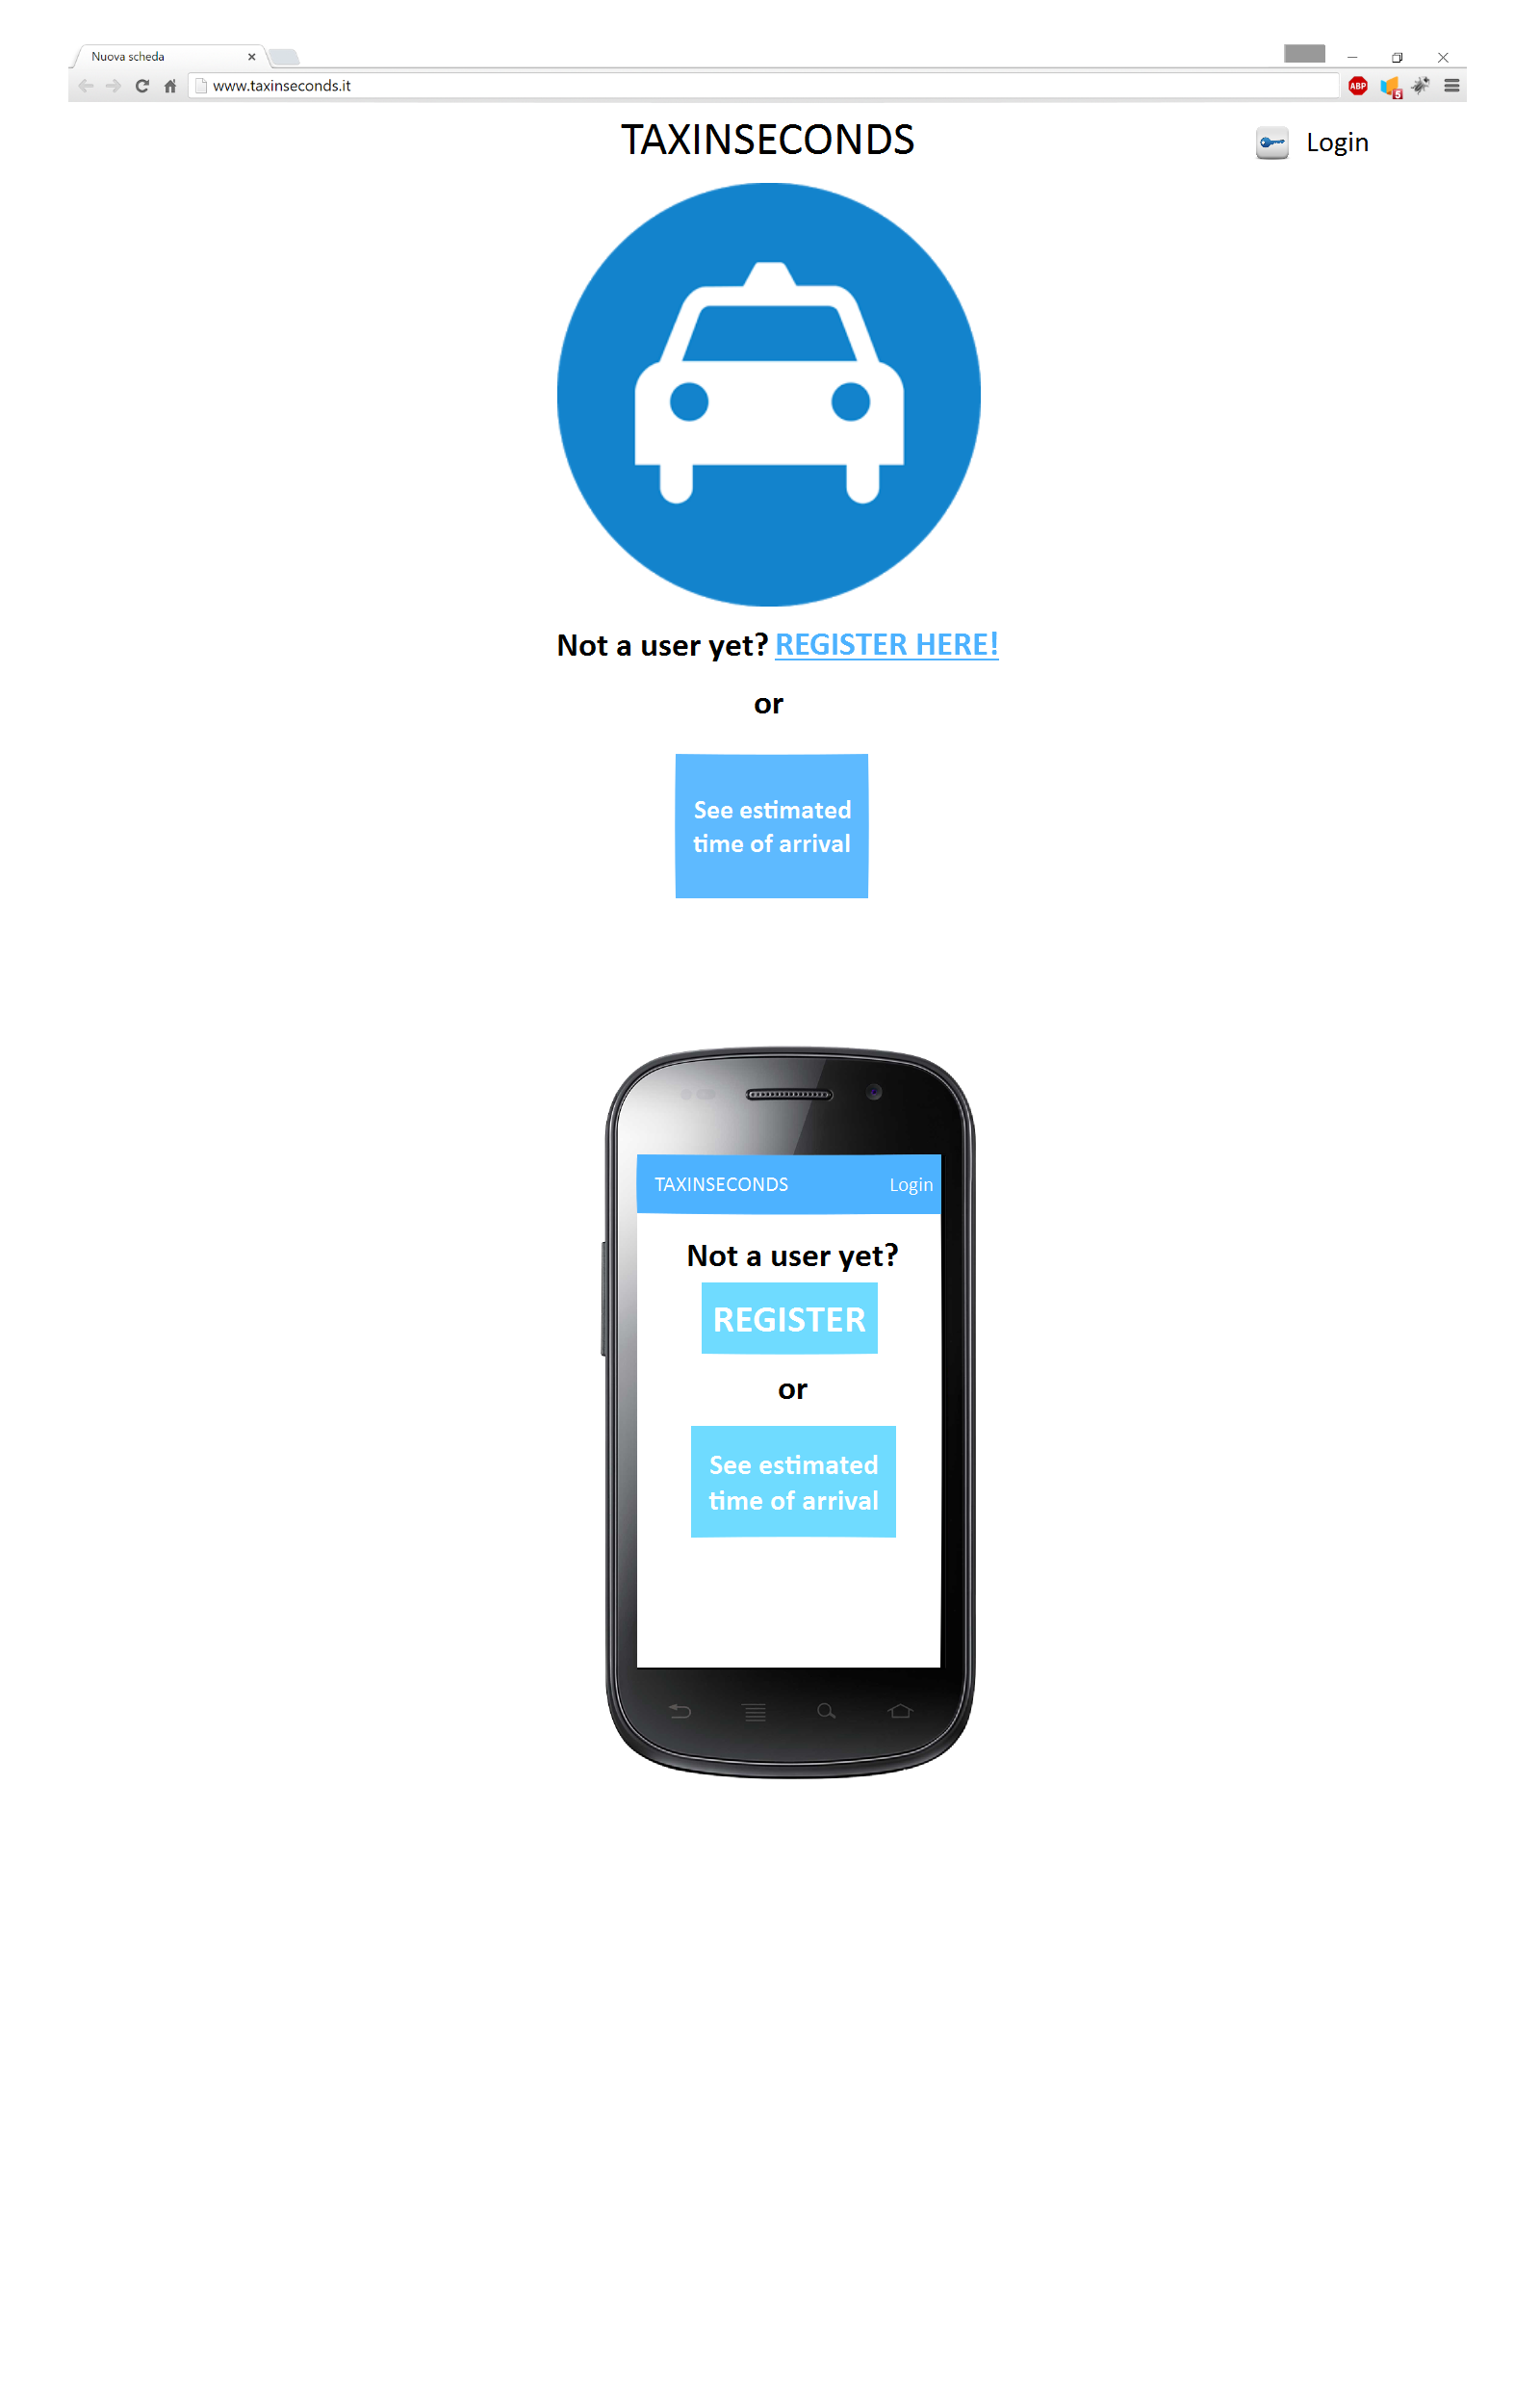
\includegraphics[width=\textwidth,height=\textheight,keepaspectratio]{GuestInterface}
	\end{center}
\end{frame}
\begin{frame}
	\frametitle{Use Cases}
	\framesubtitle{All the actions allowed were planned and analysed}
	\begin{center}
		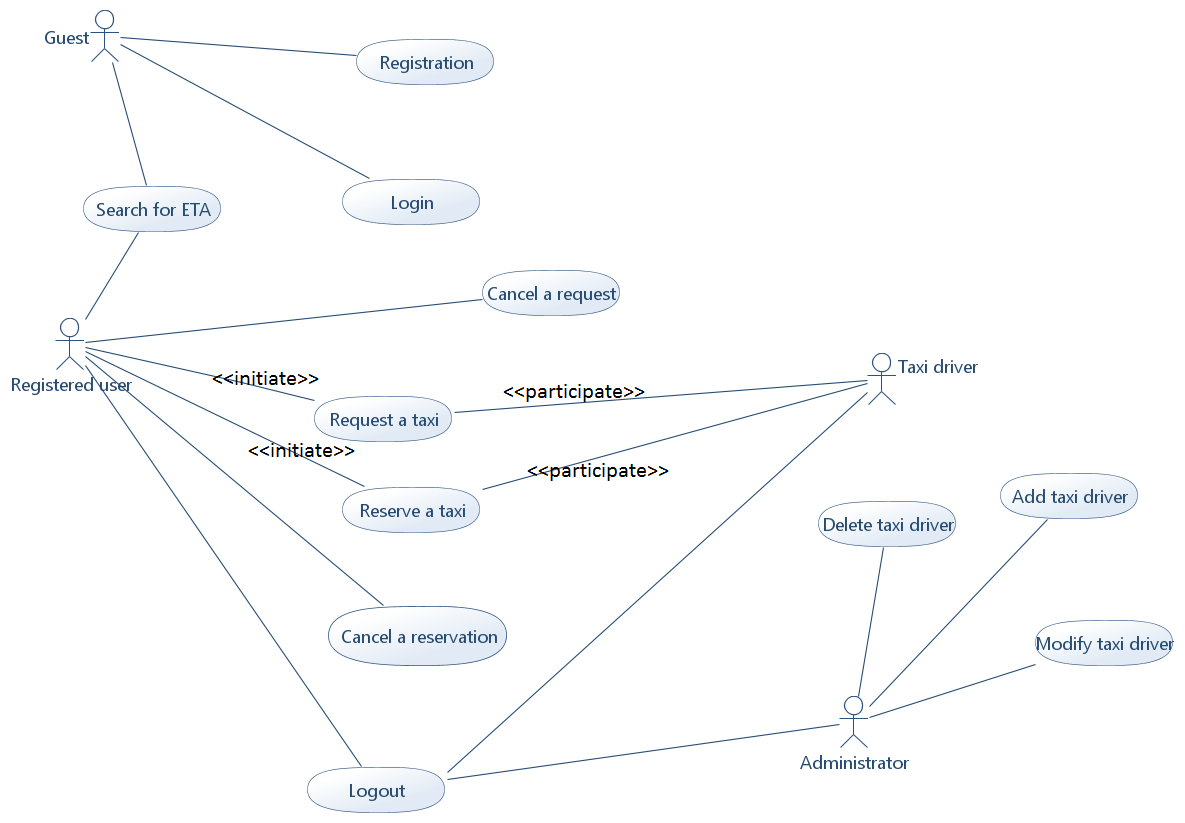
\includegraphics[width=\textwidth,height=\textheight,keepaspectratio]{UseCaseDiagram}
	\end{center}
\end{frame}
\begin{frame}
	\frametitle{Use Cases}
	\framesubtitle{Each use case is analysed in depth with a sequence diagram}
	\begin{center}
		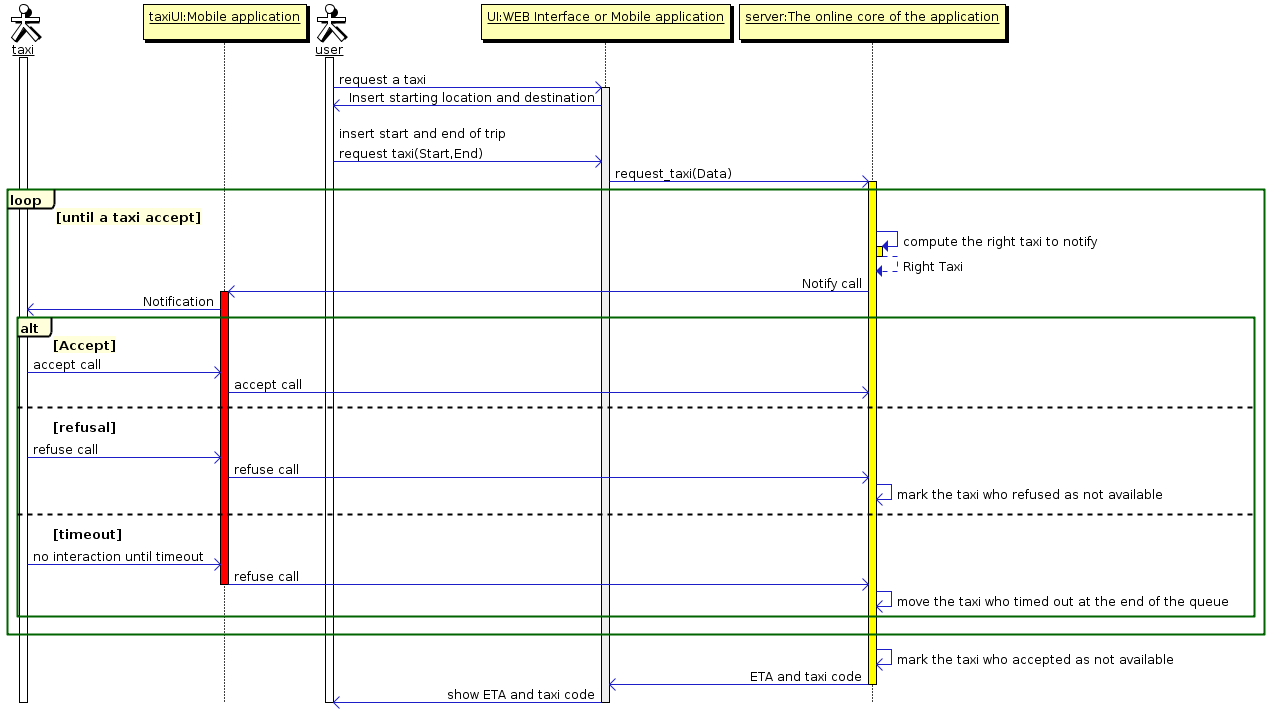
\includegraphics[width=\textwidth,height=\textheight,keepaspectratio]{request-a-taxi}
	\end{center}
\end{frame}
\begin{frame}
	\frametitle{Class Diagram}
	\framesubtitle{The class diagram was kept as readable as possible, underlying the main decisions taken}
	\begin{center}
		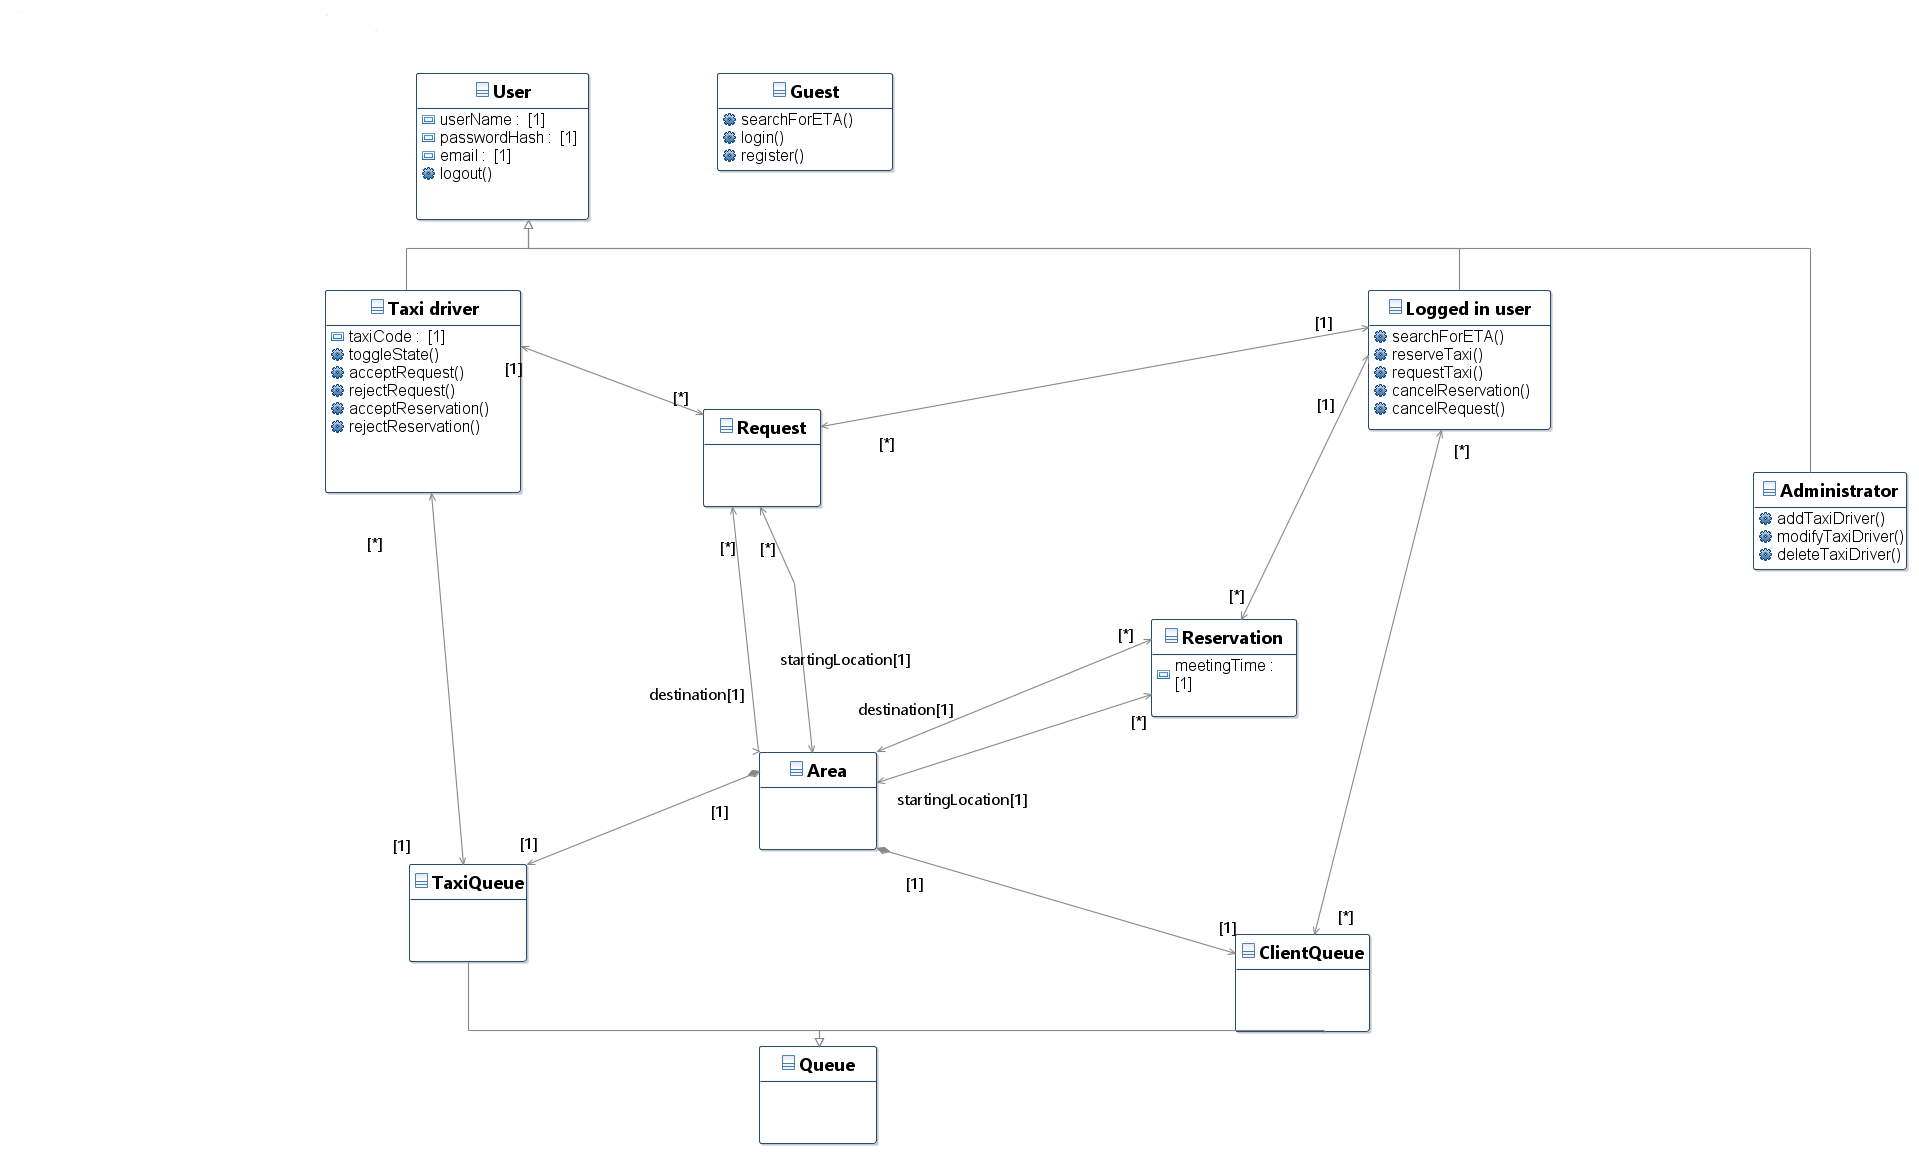
\includegraphics[width=\textwidth,height=\textheight,keepaspectratio]{ClassDiagram}
	\end{center}
\end{frame}
\begin{frame}
	\frametitle{Alloy}
	\begin{center}
		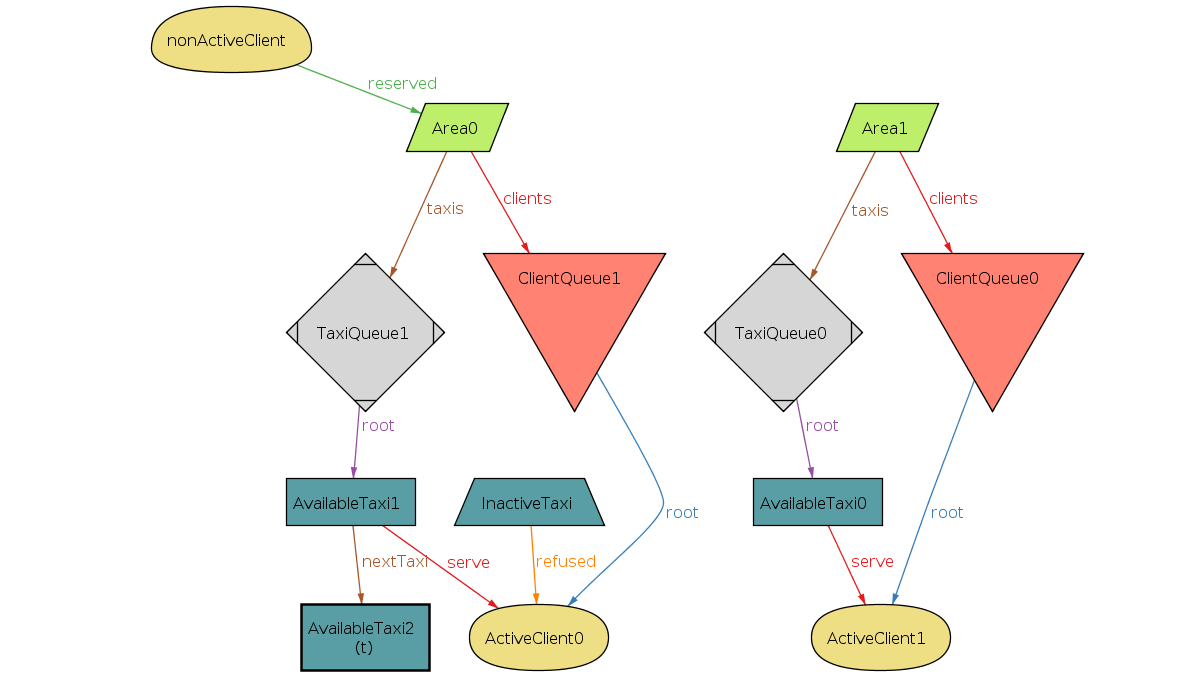
\includegraphics[width=\textwidth,height=\textheight,keepaspectratio]{reserved-and-refused}
	\end{center}
\end{frame}

\section[Section]{Design Document}
\begin{frame}
	\begin{center}
		Design Document
	\end{center}
\end{frame}
\begin{frame}
	\frametitle{The Design}
	The architecture of the application is pretty standard
	\begin{itemize}
		\item Classical DMZ structure for the Network 
		\item Database + Web server for the components
	\end{itemize}
\end{frame}
\begin{frame}
	\frametitle{The Deployment}
	\framesubtitle{A standard DMZ + Internal network approach was used}
	\begin{center}
		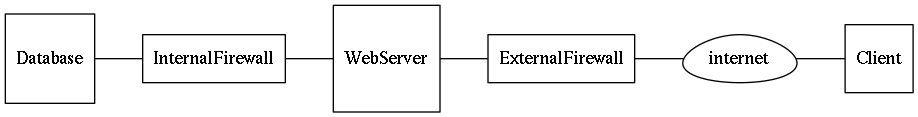
\includegraphics[width=\textwidth,height=\textheight,keepaspectratio]{dot/deployment}
	\end{center}
\end{frame}
\begin{frame}
	\frametitle{The Component View}
	\begin{center}
		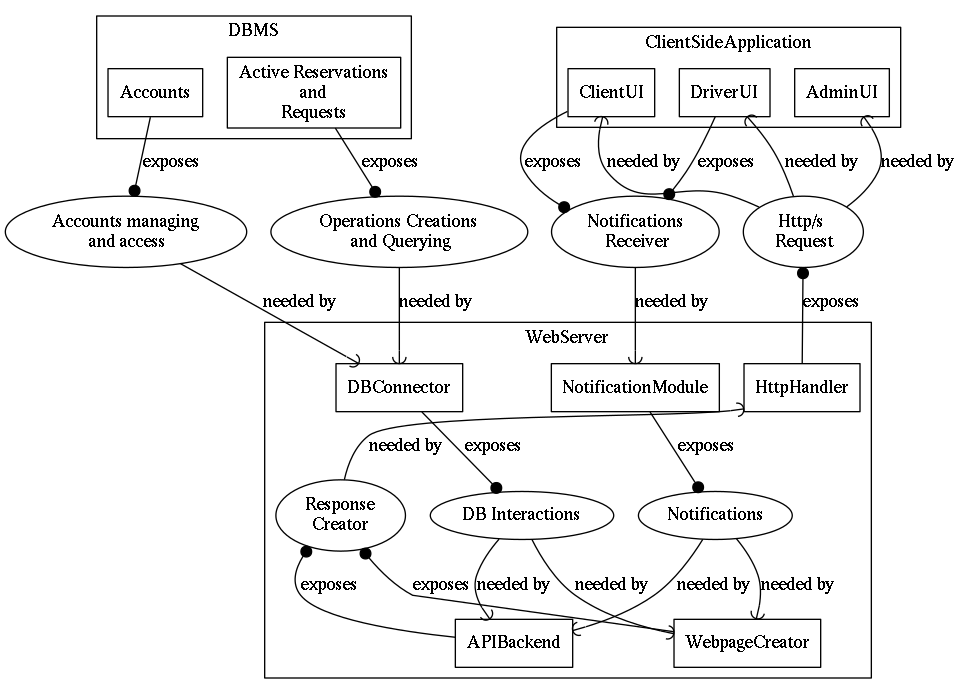
\includegraphics[width=\textwidth,height=\textheight,keepaspectratio]{dot/component}
	\end{center}
\end{frame}
\begin{frame}
	\frametitle{More on the Components}
	\framesubtitle{Extensibility and maintainability as targets}
	\begin{itemize}
		\item Both mobile and web version are based on web technologies.
		\item The queues, reservations and requests are computed by the DBMS.
		\item The web server ignores the fact that the client is using a mobile app or a browser.
		\item The APIs query the DBMS in the exact same way the Web Server does.
	\end{itemize}
\end{frame}

\section[Section]{Test Document}
\begin{frame}
	\begin{center}
		Test Document	
	\end{center}
\end{frame}
\begin{frame}
	\frametitle{The sandwich approach}
	\framesubtitle{}
	The sandwich approach allows to first test the outer parts of the applications
\end{frame}

\section[Section]{Project Plan}
\begin{frame}
	\begin{center}
		Project Plan
	\end{center}
\end{frame}
\begin{frame}
	\frametitle{Function Points}
	152 FP in Total:
	\begin{itemize}
		\item Internal Logical File 45 FP
		\item External Input 70 FP
		\item External Output 19 FP
		\item External Inquiry 18 FP
	\end{itemize}
\end{frame}
\begin{frame}
	\frametitle{COCOMO}
	\framesubtitle{}
	\begin{itemize}
		\item \textasciitilde7000 estimated thousands of \textbf{S}ource \textbf{L}ines \textbf{O}f \textbf{C}ode
		\item \textasciitilde25 Person-Month
		\item 3 People for a total of 10 Months
	\end{itemize}
\end{frame}

\section[Section]{Code Inspection}
\begin{frame}
	\begin{center}
		Code Inspection
	\end{center}
\end{frame}
\end{document}

\begin{frame}
	\frametitle{}
	\framesubtitle{}
\end{frame}
